%
% File coling2018.tex
%
% Contact: zhu2048@gmail.com & liuzy@tsinghua.edu.cn
%% Based on the style files for COLING-2016, which were, in turn,
%% Based on the style files for COLING-2014, which were, in turn,
%% Based on the style files for ACL-2014, which were, in turn,
%% Based on the style files for ACL-2013, which were, in turn,
%% Based on the style files for ACL-2012, which were, in turn,
%% based on the style files for ACL-2011, which were, in turn, 
%% based on the style files for ACL-2010, which were, in turn, 
%% based on the style files for ACL-IJCNLP-2009, which were, in turn,
%% based on the style files for EACL-2009 and IJCNLP-2008...

%% Based on the style files for EACL 2006 by 
%%e.agirre@ehu.es or Sergi.Balari@uab.es
%% and that of ACL 08 by Joakim Nivre and Noah Smith

\documentclass[11pt]{article}
\usepackage{coling2018}
\usepackage{times}
\usepackage{url}
\usepackage{latexsym}
 \usepackage{graphicx}
%\documentclass{llncs}
%\setlength\titlebox{5cm}

% You can expand the titlebox if you need extra space
% to show all the authors. Please do not make the titlebox
% smaller than 5cm (the original size); we will check this
% in the camera-ready version and ask you to change it back.

%\begin{document}
\title{STEVENDU2018's system in VarDial 2018: Discriminating between Dutch and Flemish in Subtitles}

\author{Steven Du \\
	{\tt\footnotesize  stevenlol@qq.com} \\
	\And
	Yuan Yuan Wang \\
	{\tt\footnotesize  circlea@sina.com} 
	%\And
	%Bing Tao Han \\
	%{\tt\footnotesize  hanbingtao@zte.com} \\
	%\And
	%Jia An Yang \\
	%{\tt\footnotesize  yangjiaan@zte.com}
	} 


%\maketitle
	
%\maketitle
\date{}

\begin{document}
\maketitle


\begin{abstract}
  This paper introduces the submitted system for team STEVENDU2018 during VarDial 2018~\cite{zampieri-EtAl:2018:VarDial} Discriminating between Dutch and Flemish in Subtitles(DFS). Post evaluation analyses are also presented. The results obtained indicate that it is a challenging task to discriminate between Dutch and Flemish.
\end{abstract}


\section{Introduction}
\label{intro}

%
% The following footnote without marker is needed for the camera-ready
% version of the paper.
% Comment out the instructions (first text) and uncomment the 8 lines
% under "final paper" for your variant of English.
% 
\blfootnote{
    %
    % for review submission
    %
    %\hspace{-0.65cm}  % space normally used by the marker
    %Place licence statement here for the camera-ready version. See
    %Section~\ref{licence} of the instructions for preparing a
    %manuscript.
    %
    % % final paper: en-uk version 
    %
    % \hspace{-0.65cm}  % space normally used by the marker
    % This work is licenced under a Creative Commons 
    % Attribution 4.0 International Licence.
    % Licence details:
    % \url{http://creativecommons.org/licenses/by/4.0/}
    % 
    % % final paper: en-us version 
    
     \hspace{-0.65cm}  % space normally used by the marker
     This work is licensed under a Creative Commons 
     Attribution 4.0 International License.
     License details:
     \url{http://creativecommons.org/licenses/by/4.0/}
}
The DFS task
%\footnote{\url{http://alt.qcri.org/vardial2018/}} 
is a supervised learning task to classify text into Dutch or Flemish. Dutch is the language spoken in the Netherlands and Flemish is a variant of Dutch language and also known as Belgian Dutch. There are 300000 labeled training data, 500 labeled development data, 20000 on-hold test data~\cite{vanderlee:2017:VarDial}. DUT in training data denotes Dutch, and BEL is the label for Flemish. F1 score is the evaluation metric.  %The ultimate goal is to discover approaches for Dutch and Flemish discriminant.

This paper is structured as follows: first, a brief training data analysis will be given. Then systems trained during the evaluation will be introduced. Finally more systems will be explored for post evaluation analysis.

\section{Data analysis}

The training data set consists of 300000 labeled sentences. After being lower cased and tokenized, the average sentence length in characters and number of words for both DUT and BEL is nearly the same. As showed in Table ~\ref{vocab}, it is a well balanced data set. It is worth to note that the two languages share 57.2\% of vocabulary.

 
\begin{table}[h]
	\centering
	
	
	\begin{tabular}{|l|r|r|}
		\hline
		
		Dialect & DUT & BEL \\ \hline
		Number of samples & 150000 & 150000  \\ \hline
		Average sentence length in characters & 187.86 & 187.90 \\ \hline
		Average number of words per sentence & 40.36 & 40.35 \\ \hline
		Unique words & 115560 & 115442 \\ \hline 
		Shared words & \multicolumn{2}{|c|}{66142}  \\ \hline
		Percentage of shared words & 57.2\% & 57.2\%  \\ \hline
	\end{tabular}
	\caption{Statistics for the training data set.}
	\label{vocab}
\end{table}

One interesting finding is that the use of punctuation is a little bit different. BEL has more commas, periods and question marks but less exclamation marks than DUT as showed in Table~\ref{punctuations}.

\begin{table}[h]
	\centering
	
	
	\begin{tabular}{|l|r|r|}
		\hline
		Dialect & DUT & BEL \\ \hline
		, & 157725 & 183736  \\ \hline
		. & 690629 & 708076 \\ \hline
		? & 118236 & 136742 \\ \hline
		! & 1450 & 110 \\ \hline 
	
	\end{tabular}
	\caption{Statistics for the punctuation in training data set.}
	\label{punctuations}
\end{table}

\section{Systems trained during evaluation}

There are two systems trained during evaluation: a bag-of-ngram model and dual convolutional neural network model.

\subsection{Bag-of-ngram}

Conventional methods for text classification apply common features such as bag-of-words, n-grams, and their TF-IDF~\cite{4811259} as input of machine learning algorithms, such as support vector machine (SVM)~\cite{10.1007/BFb0026683}, logistic regression~\cite{004017007000000245}, naive Bayes (NB)~\cite{Mccallum1998A} for classification.

In this work, the bag-of-ngram system and Linear SVM are used as the baseline system. First the text is lower-cased and converted to n-gram word tokens (\textit{n} is from 1 to 3), then filtered by TF-IDF with minimal document frequency of 5. Extracted features are utilized to train Linear SVM classifier. A 20 folds cross validation is performed on the training set, the average F1 score is 0.63. This system obtains 0.69 on development set. 



\subsection{Dual-CNN}
\label{sect:pdf}

This approach builds simple CNN model (with pre-trained embedding) for each language. The input text will pass through these CNNs separately. Outputs of two CNN networks are then concatenated together. This is followed by a fully connected layer for classification task. Detail of this network can be found in Figure~\ref{fig:dualcnn}, in which we limit the length of input word tokens to 60. During evaluation the proposed Dual-CNN network obtained 0.62 through cross validation and 0.61 on the development set.
\begin{figure}[h]
	\centering
	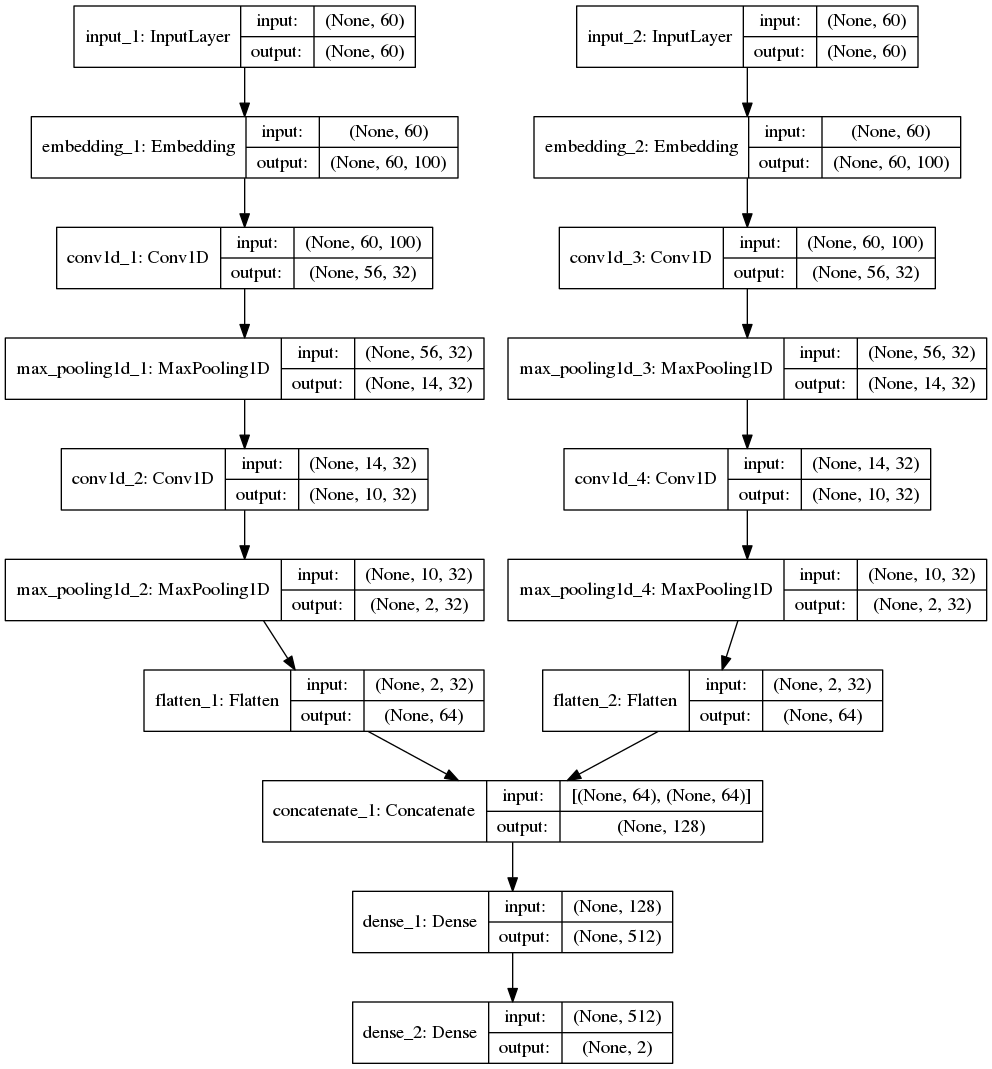
\includegraphics[width=10cm]{../../images/getDUALCNN.png}
	\caption{Proposed Dual-CNN architecture} 
	
	\label{fig:dualcnn} 
\end{figure} 
The final submitted system is only a bag-of-ngram model which has better performance than Dual-CNN.




\subsection{Evaluation results}

The score on the released test set range from 0.55 to 0.66 in Table~\ref{my-label}, our bag-of-ngram, the most simple approach yields 0.623. On the other hand the proposed Dual-CNN yields 0.621. The test score correlated well with the local cross validation score, development set is not the right choice for model selection. The best score is just 0.66, which implies that the DFS task is challenging.

\begin{table}[h]
	\centering

	\begin{tabular}{|l|l|l|l|}
		%\cline{1-3}
		 \hline
		Rank & Team         & Run & F1 (macro)     \\  \hline
		1    & Tübingen-Oslo & 3   & 0.6600474291   \\  \hline
		2                          & Taurus                            & 4                        & 0.6455823383   \\  \hline
		3                          & clips                             & 2                        & 0.6357352338   \\  \hline
		3                          & LaMa                              & 3                        & 0.6325606971   \\ \hline
		3                          & XAC                               & 3                        & 0.6317829736   \\ \hline
		3                          & safina                            & 0                        & 0.6308914957   \\ \hline
		4                          & \textbf{STEVENDU2018}                      & 2                        & \textbf{0.6230923676}   \\ \hline
		4                          & mskroon                           & 5                        & 0.6201248435   \\ \hline
		5                          & SUKI                              & 1                        & 0.6127429864   \\ \hline
		6                          & DFSlangid                         & 3                        & 0.5961836466   \\ \hline
		7                          & dkosmajac                         & 1                        & 0.5674320041   \\ \hline
		7                          & benf                              & 2                        & 0.5582862249   \\  \hline
	\end{tabular}	
	\caption{Evaluation results}
	\label{my-label}
\end{table}

\section{Post evaluation systems}
Since the bag-of-ngram system only scores 0.623 on test set, to achieve better result a series of studies had been carry out after the evaluation. These can be broadly divided into three groups: one group focus on finding the vector representation for the given text data, another group focus on deep learning approaches, third group utilize existing text classification framework. % the last group intend to solving DFS challenge via data augmentation.



\subsection{Vector representation based approach}

Vector representation approach intends to convert text data in variable-length pieces of text into a fixed-length low dimension vector. There are many works have been done in this direction~\cite{2014arXiv1408.5882K,2015arXiv151108198W,Kusner2015From,Kenter2016Siamese,Ye2017Determining}, only two basic approaches are investigated here: by taking mean value of word vectors and through doc2vec from the work in distributed representation of sentences and documents~\cite{Le2014Distributed}. 

\subsubsection{Mean word vector system}
A popular idea in modern machine learning is to represent words by vectors. These vectors capture hidden information about a language, like word analogies or semantics. Commonly used word vectors are word2vec~\cite{Mikolov2013Distributed}, Glove~\cite{Pennington2014Glove} and fastText~\cite{bojanowski2017enriching}. FastText is capable to capture sub-word information, thus in this study, we use FastText to train word vectors. Skip-gram, window size of 5 and minimal word count of 5, 5 negative samples, sub-word range is between 3 and 6 characters are the default training parameters. After training, for each sentence, the mean value of its word vectors is used as feature, Linear Discriminant Analysis classifier\footnote{\url{http://scikit-learn.org/stable/modules/lda_qda.html}} is selected as the learning algorithm.

\begin{table}[h]
	\centering
	
	
	\begin{tabular}{|l|l|l|l|l|l|}
		\hline
		Word vector dimension & 40 & 100 & 250 & 300 & 400 \\ \hline
		Test F1 Score & 0.5642 & 0.5848 & 0.5922 & 0.598 & 0.6024 \\ \hline
	\end{tabular}
	\caption{F1 scores for mean word vector system}
	\label{word2vec}
\end{table}

Table~\ref{word2vec} shows F1 score for the mean word vector system. With increase in the number of dimensions, the system performance improved.\label{vectorsize} % The 400 dimensional word vector is suitable for this task..


\subsubsection{Doc2vec}

In this study we use the doc2vec~\cite{Le2014Distributed} from gensim\footnote{\url{https://radimrehurek.com/gensim/index.html}}. The doc2vec model is trained on training data set with minimal word occurrence of 5 and window size of 8. Table~\ref{doc2vec} shows the best score is 0.5308, which is slightly better than random guess.

\begin{table}[h]
	\centering
	
	
	\begin{tabular}{|l|l|l|l|}
		\hline
		Sentence vector dimension & 100 & 200 & 300 \\ \hline
		Test F1 Score & 0.5282 & 0.5246 & 0.5308 \\ \hline
	\end{tabular}
	\caption{F1 scores for Doc2vec}
	\label{doc2vec}
\end{table}




Two sets of sentence vector have been evaluated in this study. The average word vector approach is better than doc2vec. In the following experiment, 400 is used as the default size of word embedding.


\subsection{Deep learning based approaches}

Our proposed Dual-CNN didn’t beat the conventional bag-of-ngram model. This motivated us to examine the performance of deep learning approaches. Five types of deep learning based approaches are investigated (all of them use word level embeddings), starting from the most basic architecture, they are:
\subsubsection{MLP}
The MLP system is built by an embedding layer, one flatten layer and fully connected layer as illustrated in Figure~\ref{fig:mlp} . Please also refer to system diagrams in github repository\footnote{\url{https://github.com/StevenLOL/vardial2018_dfs_stevendu2018}}.
\begin{figure}[h]
	\centering
	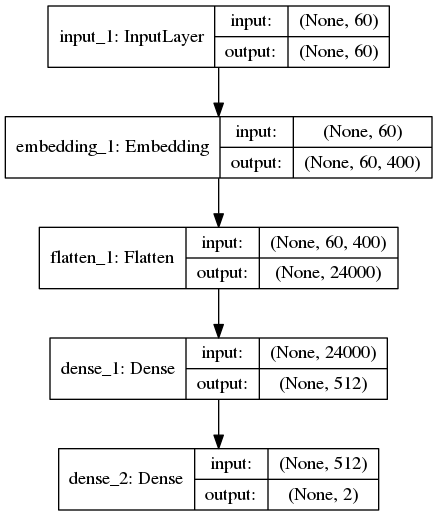
\includegraphics[height=6.5cm]{../../images/getMLP.png}
	\caption{MLP architecture} 
	
	\label{fig:mlp} 
\end{figure} 
 
\subsubsection{AVERAGE}
The AVERAGE system is similar to MLP system but the flatten layer is replaced by an average pooling layer. It is also known as neural bag-of-word model and being surprisingly effective for many tasks~\cite{Iyyer2015Deep}. 
\subsubsection{GRU}  
The GRU system is similar to AVERAGE system but the average pooling layer is replaced by a bidirectional GRU layer.
\subsubsection{CNN-LSTM} 
The CNN-LSTM system is built by an embedding layer followed by two convolution-max pooling layers and one bidirectional GRU layer.

These four deep approaches are indeed the most fundamental networks in NLP research. Incorporating language model fine-tunning~\cite{2018arXiv180106146H} and attention mechanism~\cite{Vaswani2017Attention} are the recent trends, which we leave them for further exploration.

\begin{table}[h]
	\centering
	
	
	\begin{tabular}{|l|l|l|l|}
		\hline
		Word Embedding & D20 Random & D400 Random & D400 pre-trained \\ \hline
		MLP & 0.6350 & \textbf{0.6365} & 0.6334 \\ \hline
		AVERAGE   & 0.6352      & 0.6356               & \textbf{0.6402}       \\ \hline
		GRU & 0.6299 & 0.6388 & \textbf{0.6413} \\ \hline
		CNN-LSTM & 0.6352 & \textbf{0.6421}  & 0.6399 \\ \hline
	\end{tabular}
	\caption{F1 scores for popular deep learning based approaches}
	\label{4deepnets}
\end{table}

Table~\ref{4deepnets} presents results for four popular deep learning based approaches. D20 Random denotes randomized word embedding of 20 dimensions. D400 pre-trained denotes embedding layer is pre-trained with word vector size of 400 dimensions. These results confirm the observation in~\ref{vectorsize}, that the 400 dimension word vectors is a good choice for this task. Three out of four systems are higher than 0.64 which are significantly better than submitted baseline system.


\subsubsection{CapsuleNet}
Capsules with transformation matrices allowed networks to automatically learn part-whole relationships. Consequently, ~\cite{2017arXiv171009829S} proposed capsule networks that replaced the scalar-output feature detectors of CNNs with vector-output capsules and max-pooling with routing-by-agreement. The capsule network has shown its potential by achieving a state-of-the-art result on highly overlapping digit parts in MutiMNIST data set. The PrimaryCapsule employed in that paper is a convolutional capsule layer with 32 channels of convolutional 8D capsules. We increase the number of channels from 32 to 320 in this study, the assumption is that there are more part-whole relations in the language than those in MNIST digit images. 


\begin{table}[h]
	\centering
	
	
	\begin{tabular}{|l|l|l|l|}
		\hline
		Number of Channels & 32 & 320 & 320 \\ \hline
		Output dimension   & 1      & 1               & 2      \\ \hline
		Test F1 Score & 0.5992 & 0.6076 & \textbf{0.6206} \\ \hline
	\end{tabular}
	\caption{CapsuleNet classification results. }
	\label{CapsuleNetTB}
\end{table}


Table~\ref{CapsuleNetTB} introduces F1 score of CapsuleNet on the test data set. The results indicate that with the increase of number of channels and thus the number of capsules, the system performed better. When changing the binary classification problem to two class classification problem, the capsule net yielded comparable result to the bag-of-ngram baseline. Work by~\cite{2018arXiv180400538Z} also shows significant improvement when transferring single-label to multi-label text classifications.




\subsection{Text Classification Framework}
FastText~\cite{joulin2016bag} is a library for efficient learning of word representations and sentence classification\footnote{\url{https://github.com/facebookresearch/fastText}}. It uses vectors to represent word n-grams to take into account local word order, which is important for many text classification problems. Following Table~\ref{fasttextClassification} shows fastText classification results. The 0.6476 is the highest score achieved.


\begin{table}[h]
	\centering
	
	
	\begin{tabular}{|l|l|l|l|}
		\hline
		Word n-gram   & 1      & 2               & 3      \\ \hline
		Test F1 Score & 0.6318 & \textbf{0.6476} & 0.6377 \\ \hline
	\end{tabular}
	\caption{FastText classification results.}
	\label{fasttextClassification}
\end{table}















%\section{Discussion}

%Language model fine-tunning~\cite{2018arXiv180106146H} and attention are two possible way to boost system performance, we will investigate in further studies. 


%\subsection{Things that not work here}


%\subsubsection{1D CNN on Character Sequence}
%\cite{8004872} propose one-dimensional convolution neural networks for encrypted network traffic classification. In which the traffic data in byte sequence are directly feed into neural networks, accuracy of 86.6 is reported on 12 classes classification task. Motivated by this, we reimplemented the 1D CNN network in both Keras and Tensorflow, the systems are first evaluated on traffic classification, 96.0 accuracy is obtained on same task. But when the same network applied to this task.  
 
%\subsubsection{More Flemish Text}

\section{Conclusion}
In this paper, a wide range of systems have been evaluated for the VarDial 2018 DFS task. A bag-of-ngram system score 0.6230 and serves as the baseline. Complex systems such as Dual-CNN and CapusleNet have competitive score to baseline system. Four simple deep learning based methods outperform baseline, three of them are higher than 0.64. FastText is identified as the best single system, yielded a F1 score of 0.6476.



% include your own bib file like this:
\bibliographystyle{acl}
%\bibliography{coling2018}

%\begin{thebibliography}{}



%\end{thebibliography}

\bibliography{cite.bib}

\end{document}
